% ICAIF 2026 submission. ACM acmart class, sigconf format.
% Compile with: pdflatex -shell-escape paper && bibtex paper && pdflatex paper && pdflatex paper

\documentclass[sigconf, anonymous, review]{acmart}

% Anonymized for review; remove `anonymous` for camera-ready.

\AtBeginDocument{%
  \providecommand\BibTeX{{%
    \normalfont B\kern-0.5em{\scshape i\kern-0.25em b}\kern-0.8em\TeX}}}

\setcopyright{none}
\acmConference[ICAIF '26]{ACM International Conference on AI in Finance}{November 2026}{TBD}

% packages
\usepackage{booktabs}
\usepackage{graphicx}
% amsmath / amssymb are already loaded by acmart; loading them again
% redefines \Bbbk and similar.
\usepackage{xcolor}
\usepackage{microtype}

\graphicspath{{../figures/}}

%==============================================================================
\title{SSL as a feature engine, not a competitor: self-supervised
pretraining for tabular credit default prediction}

\author{Anonymous Author(s)}
\affiliation{%
  \institution{Anonymous Institution}
  \country{}}
\email{anon@example.com}

%==============================================================================
\begin{document}

\begin{abstract}
Default prediction in consumer credit is dominated in practice by
gradient boosting machines (GBM) trained on hand-crafted aggregated
features --- decades of domain knowledge encoded into the data
pipeline. Self-supervised pretraining (SSL) has powered representation
learning in NLP and vision, but reports of whether it ``beats GBM'' in
credit risk are inconsistent across studies, and the reasons are
under-decomposed. We study a single public dataset
(AMEX Default Prediction; 458{,}913 customers $\times$ up to 13 months
of anonymized statements) on a single 8\,GB laptop GPU, with a fixed
customer-level 80/10/10 split, the official AMEX competition metric,
and a shared 4-layer transformer encoder backbone (869K parameters).
We train four SSL objectives (masked feature modeling, next-step
prediction, contrastive, hybrid) and compare them across three axes:
\emph{evaluation protocol} (linear probe vs.\ full fine-tune),
\emph{label budget} (1\%--100\%), and \emph{feature fusion}
(SSL embedding as additional GBM input). Four findings.
(1)~No standalone SSL model beats a tuned LightGBM baseline
(test AMEX 0.7956); the best SSL alone reaches 0.7927.
(2)~Linear probe and full fine-tune of the same encoder disagree by
0.058 in test AMEX, suggesting that prior tabular SSL benchmarks are
critically protocol-underspecified.
(3)~Treating the 128-dim SSL embedding as an auxiliary GBM feature
yields a robust improvement of $+0.00142 \pm 0.0006$ (mean over
3 pretrain seeds, $t = 4.1$, all 3 trials positive) over the
baseline; the best single seed reaches $0.79768$ ($+0.00210$).
(4)~The lift is targeted, not uniform: it concentrates in the bottom
deciles of GBM's base prediction ($+0.02$ to $+0.03$ per decile),
the region operationally most exposed to false-negative risk. An
ablation shows SSL embeddings recover $\approx 55\%$ of the
predictive signal lost by removing the top-100 hand-crafted
features. Multi-encoder stacking exhibits negative scaling.
We conclude that, on this dataset, SSL is best framed not as a
competitor to but as an \emph{auxiliary feature engine for} a
GBM-based credit-risk pipeline, with value concentrated in the
operationally critical false-negative tail.
\end{abstract}

\keywords{self-supervised learning, credit risk, gradient boosting,
tabular data, evaluation protocols}

\maketitle

%==============================================================================
\section{Introduction}
\label{sec:intro}

\paragraph{Industry standard and its limits.}
Consumer credit default prediction is among the longest-studied applied
statistics problems, and the industry standard over the past decade is
unambiguous: \emph{gradient boosting machines (GBM) trained on
hand-crafted aggregated features}. Practitioners compress
transaction-level sequences --- often spanning years and hundreds of
millions of statements --- into customer-level row vectors via
hand-engineered aggregators such as ``last value over 12 months,''
``standard deviation of utilization,'' ``trend slope of balance,'' and
hundreds of similar transformations. The result, fed to LightGBM or
XGBoost, defines the dominant credit-risk pipeline in industry and
sweeps the top of public credit-risk benchmarks: nearly every top
solution to the AMEX Default Prediction Kaggle Challenge of 2022
followed exactly this pattern~\cite{AMEX_1st_place_2022}. Our own
reproduction reaches OOF AMEX 0.79222 and test bagged AMEX 0.79558
with $1{,}291$ hand-crafted features, placing it in the public
leaderboard top-10 range.

This baseline embeds two facts. First, \emph{decades of domain
knowledge are effectively pretrained into the data pipeline itself}
--- a new model has to lift over a system in which expert priors are
already compiled into the inputs. Second, the temporal structure of
the raw sequence is irreversibly compressed by hand-chosen
aggregators; what information is lost in that compression is rarely
quantified.

\paragraph{NLP/Vision SSL successes and credit-domain ambiguity.}
Self-supervised pretraining (SSL) has been the dominant
representation-learning recipe in natural language
processing~\cite{Devlin2018,Radford2018} and computer
vision~\cite{Chen2020,He2022_MAE}: representations pretrained without
labels on raw signal outperform hand-crafted features once enough data
and compute are present. The natural conjecture is that the same
recipe should transfer to credit risk. Several lines of
work~\cite{Babaev2019,Padhi2021,Skentzos2022} have claimed exactly
this, arguing that pretrained sequence encoders over transactions can
beat the GBM standard.

The literature, however, is inconsistent. Across comparable model
families and dataset sizes, some studies report SSL beating GBM and
others report the opposite, and the conditions separating the two
outcomes are not systematically decomposed. In our own experiments on
a single fixed customer-level split, with the same encoder backbone
and the same metric, \emph{changing the downstream evaluation protocol
alone moves the AMEX metric by 0.058} (from $-0.058$ to $-0.003$
relative to baseline). That gap is wider than the spread between
``SSL barely loses'' and ``SSL is hopeless,'' yet it is rarely reported.

Our starting position is therefore that \emph{``does SSL work on
credit?''} is the wrong question; the right question is \emph{``under
which evaluation protocol, at which label budget, and under which
feature-fusion scheme does SSL produce a measurable lift over a strong
GBM baseline?''} We decompose this with a single-environment
controlled study.

\paragraph{Our approach.}
We use the public AMEX Default Prediction dataset~\cite{Kaggle2022}
($458{,}913$ customers $\times$ up to 13 months of anonymized
statements) on a single RTX 4070 Laptop GPU (8\,GB VRAM) and vary
three axes while holding all other choices fixed:
\begin{itemize}
  \item \textbf{Evaluation protocol.} For the same pretrained encoder
        we report both (a) \emph{linear probe} --- encoder frozen,
        mean-pool features fed to a logistic regression --- and
        (b)~\emph{full fine-tune} of the encoder plus a classification
        head.
  \item \textbf{Label budget.} We compare GBM and SSL fine-tune over
        stratified subsets of $1\%$, $5\%$, $25\%$, and $100\%$ of the
        labeled pool.
  \item \textbf{Feature fusion.} We extract mean-pooled SSL embeddings
        for every customer and concatenate them with the hand-crafted
        feature set fed to GBM. We measure the marginal lift and
        decompose where it lives via ablation and segment analysis.
\end{itemize}
All four SSL objectives we consider --- masked feature modeling
(BERT-style), next-step prediction (GPT-style), SimCLR-style
contrastive learning, and a masked\,+\,contrastive hybrid --- share
the same 4-layer transformer encoder backbone with $d_{\text{model}}
= 128$ and $852{,}544$ parameters. All experiments use the same
customer-level $80/10/10$ split fixed by seed and stored on disk with
a verified SHA-256 hash.

\paragraph{Contributions.}
We make four contributions, each numerically supported.

\begin{itemize}
  \item \textbf{Direct competition.} No single SSL configuration we
        tried beats the LightGBM baseline at test AMEX $0.7956$. The
        best SSL alone, hybrid + full fine-tune, reaches $0.7927$
        ($-0.003$). Moreover, in a few-shot study GBM strictly
        dominates SSL at every labeled fraction, with the gap
        \emph{widening} as labels shrink ($+0.052$ at 1\%) ---
        contrary to the standard ``SSL is label-efficient'' framing.
  \item \textbf{Protocol gap.} Linear probe and full fine-tune of the
        same pretrained encoder disagree by $0.058$ in test AMEX. The
        ranking of the four SSL objectives \emph{reverses} between
        the two protocols. We argue that prior tabular SSL evaluations
        are critically under-specified: any claim of the form ``SSL
        $A$ outperforms SSL $B$'' is protocol-conditional and must
        report both numbers.
  \item \textbf{Feature fusion.} Treating a single SSL encoder's
        128-dim mean-pooled embedding as additional input features to
        GBM yields a robust improvement of $+0.00142 \pm 0.0006$
        (mean of three SSL pretrain seeds, $t = 4.1$, df $= 2$, all
        three trials positive) in test bagged AMEX over the GBM
        baseline; the best single seed reaches $0.79768$.
  \item \textbf{Localized lift.} The improvement is concentrated in
        the bottom four deciles of GBM's base prediction --- the
        ``GBM thinks this customer is safe'' region --- at
        $+0.02$ to $+0.03$ per decile. The SSL embedding flags
        \emph{silent default risk} in confident-safe customers, the
        most operationally costly false-negative failure mode. An
        ablation further shows that the SSL embedding recovers
        $\approx 55\%$ of the predictive content of the top-100
        hand-crafted features when those features are removed, and
        multi-encoder stacking exhibits negative scaling --- the NLP
        and vision SSL intuition that ``more pretraining objectives
        yield more signal'' does not transfer to tabular credit at
        this scale.
\end{itemize}

Taken together, these findings reposition SSL in tabular credit risk
not as a competitor to but as an \emph{auxiliary feature engine for}
the prevailing GBM pipeline. We make this concrete with deployment
guidance in Section~\ref{sec:discussion}.

%==============================================================================
\section{Related work}
\label{sec:related}

\paragraph{Sequence modeling and SSL in credit risk.}
Two threads run through the recent credit-risk literature on sequence
models. \emph{Supervised end-to-end} approaches train RNN/LSTM or
transformer backbones directly on customer-level binary default labels.
Sberbank's E.T.-RNN~\cite{Babaev2019} trained an LSTM on transactions
and reported improvements over a logistic regression baseline. The
limitation is the choice of comparator: their baseline is not the
hand-crafted-feature GBM that dominates industry practice, and direct
comparisons of sequence models to such GBMs have not consistently
favored the deep approach~\cite{Sirignano_mortgage,Khandani2010}.

\emph{Pretraining-based} approaches are closer to our framing.
Padhi~et~al.~\cite{Padhi2021} introduced TabBERT and TabGPT, applying
masked feature modeling and next-step prediction to credit transaction
sequences. Their results on fraud and default tasks include conditions
in which SSL representations match or exceed hand-crafted features, but
evaluations are conducted under a single protocol (linear probe
\emph{or} fine-tune, not both), so cross-protocol consistency is not
established. Skentzos~et~al.~\cite{Skentzos2022} apply sequence models
in credit contexts without pretraining. We are not aware of a published
work that (i)~uses a shared backbone, (ii)~holds the dataset split
fixed, and (iii)~varies SSL objective, evaluation protocol, label
budget, and feature-fusion scheme simultaneously, in a single
controlled study on credit risk.

\paragraph{General tabular SSL.}
Tabular SSL outside the credit domain has been studied through value
imputation~\cite{VIME2020}, feature corruption with contrastive
learning~\cite{SCARF2021}, and row-attention with
contrastive pre-training~\cite{SAINT2022}. These works largely target
short row-wise tabular benchmarks where there is no per-customer
temporal axis, and their comparisons to GBM on identical
hand-crafted features are uneven. Credit transaction sequences differ
in two relevant respects: the temporal axis is explicit but short
(typically $\leq 13$ statements), and the feature schema is wide but
not language-like. NLP long-sequence assumptions and vision
dense-grid assumptions both transfer imperfectly to this regime.

\paragraph{Evaluation-protocol gaps.}
That linear probe and full fine-tune can disagree is well known in
NLP and vision~\cite{Chen2020,He2022_MAE}; the standard practice is to
report both and treat the gap as an indicator of representation
linear-separability versus end-to-end trainability. In the
tabular-credit literature this practice is rarely followed. To our
knowledge, no prior credit-SSL paper reports both protocols, on the
same backbone, on the same split, in a single results table. We argue
in Section~\ref{sec:results} that this omission is responsible for
substantial cross-paper inconsistency in the field.

\paragraph{Deep representations as GBM features.}
The idea of stacking neural network outputs as additional GBM inputs
is a standard Kaggle-style ensembling tactic and has been reported in
auto insurance~\cite{Kang2022} and fraud detection~\cite{Lopez2020}.
These reports state aggregate performance gains but rarely decompose
\emph{what} deep features add to hand-crafted ones, \emph{which
customer segments} benefit, or how marginal value scales with
ensemble size. We are not aware of a controlled study of these
questions in the credit-sequence setting. Section~\ref{sec:results}
fills these gaps.

%==============================================================================
\section{Data and setup}
\label{sec:setup}

\paragraph{Dataset.}
We use the public AMEX Default Prediction Kaggle
Challenge~\cite{Kaggle2022}: $458{,}913$ customers, each with up to
13 monthly statements of anonymized transaction features. Each
statement carries roughly 188 numerical and 11 categorical anonymized
columns plus a statement date \texttt{S\_2}. The customer-level binary
label encodes whether the customer defaults within 18 months of their
last observed statement. The base default rate is approximately
$26\%$, and some customers have shorter histories (cold-start).
The data is anonymized, so domain interpretation is limited, but
since the goal of this work is methodological --- a controlled
comparison of evaluation regimes --- anonymization does not
materially affect the conclusions.

\paragraph{Customer-level 80/10/10 split.}
All experiments use the same customer-level $80/10/10$ stratified
split. We employ \texttt{StratifiedShuffleSplit} with seed $42$ to
carve test (10\%) and val (10\%) out of the labeled pool, and
\texttt{StratifiedKFold} within the train+val pool to produce a fixed
5-fold index. The result is stored at
\texttt{data/splits/v1.parquet} and verified with SHA-256: a fresh
generation produces a byte-identical artifact. All Phase 1--5
experiments read this single artifact.

\paragraph{Evaluation metric.}
The official AMEX competition
metric~\cite{RohanRao_metric} is
\(M = \tfrac{1}{2}(G + D)\), where $G$ is a normalized weighted Gini
coefficient with the negative class weighted by 20 (to correct for
downsampling in the public dataset), and $D$ is the default rate
captured among the top $4\%$ of predictions by cumulative weight. We
re-implemented $M$ in NumPy and validated it against a slow pandas
oracle on nine unit tests: the two implementations agree to within
$10^{-9}$ on perfect, inverse, random, and noisy-realistic inputs,
and on permutation invariance, input validation, and tie handling.
Beyond AMEX $M$ we also report AUC, KS, and log-loss throughout.

\paragraph{LightGBM baseline.}
The Phase 1 baseline is a 5-fold cross-validated LightGBM trained on
$1{,}291$ customer-level hand-crafted features. The feature recipe
follows the conventions of the AMEX 2022
top solutions~\cite{AMEX_1st_place_2022}: for each numerical column we
compute \{last, mean, std, min, max, last$-$first diff, last/mean
ratio\}; for each categorical column \{last, n\_unique, count, mode\};
plus 3 missing-pattern aggregates and 5 statement-gap aggregates.
Hyperparameters follow the public 1st-place writeup
(\texttt{learning\_rate=0.01}, \texttt{num\_leaves=100},
\texttt{min\_child\_samples=2400}, \texttt{reg\_alpha=0.5},
\texttt{reg\_lambda=0.5}, \texttt{colsample\_bytree=0.4},
\texttt{subsample=0.8} with frequency~5, \texttt{max\_bin=255},
$10{,}500$ rounds with $200$-round early stopping); the AMEX metric is
registered as a custom \texttt{feval} so that early stopping responds
to the task metric. The model reaches OOF AMEX $0.79222$ and test
bagged AMEX $0.79558$, which is in the public leaderboard top-10
range and serves as the reference for every subsequent comparison.

\paragraph{Compute.}
All experiments ran on a single laptop --- NVIDIA RTX 4070 Laptop GPU
(8\,GB VRAM, sm\_89), AMD Ryzen 9 7940HS (16 logical cores), 32\,GB
RAM. SSL pretraining used PyTorch 2.6.0+cu124 and PyTorch Lightning
2.6.4 with bf16 mixed precision; LightGBM used all CPU cores. No
cloud GPU was used. The total compute across all 5 phases was
approximately 20--22 GPU+CPU-hours. The single-laptop reproducibility
of this study lowers the barrier for individual credit-risk data
scientists to evaluate SSL on their own data, in contrast to
NLP-style SSL benchmarks that require multi-GPU clusters.

%==============================================================================
\section{Methods}
\label{sec:methods}

\subsection{Shared transformer encoder}
\label{sec:enc}

All four SSL objectives share an identical encoder backbone, ensuring
that performance differences are attributable to objective choice
and not to architecture confounders.

\paragraph{Feature embedder.}
Each statement carries $F_{\text{num}} = 177$ numerical features,
$F_{\text{cat}} = 11$ categorical columns, and a missingness
indicator. Numerical inputs are z-score normalized using means and
standard deviations computed on the \emph{train} split only;
missing entries are replaced with $0$ and concatenated with a $0/1$
missingness mask, so the numerical branch input dimension is
$2F_{\text{num}}$, projected to $d_{\text{model}} = 128$ by a single
linear layer. Each categorical column has its own small embedding
table (\texttt{padding\_idx} $= 0$ reserves a MISSING/unknown token);
all category embeddings (each of dimension $d_{\text{cat}} = 8$) are
concatenated across columns and projected to $d_{\text{model}}$ by
another linear layer. The output timestep representation is the sum
of the two branches, of shape $(B, T, D) = (B, 13, 128)$.

\paragraph{Positional encoding and CLS token.}
Because sequences are short ($T \leq 13$) we use a learned positional
embedding parameter rather than a sinusoidal one. Masked,
contrastive, and hybrid objectives prepend a learned CLS token to
the sequence, producing $(B, T+1, D)$; the CLS slot serves as the
sequence-level summary. Next-step prediction does not use a CLS
token to keep the causal structure clean.

\paragraph{Transformer.}
A 4-layer Pre-LN~\cite{Xiong2020} transformer encoder with $8$ heads
of dimension $32$, feed-forward dimension $512$, GELU activation, and
dropout $0.1$. Padding is blocked by the attention mask, and an
additional causal mask is applied for next-step prediction. The
encoder has $852{,}544$ parameters; full objective modules (including
heads) total $869$K--$915$K parameters depending on the objective.

\subsection{Four SSL objectives}
\label{sec:obj}

\paragraph{Masked Feature Modeling (MFM).}
BERT-style masking~\cite{Devlin2018} adapted to tabular shape. In each
batch we randomly sample $15\%$ of (timestep, feature) cells: numerical
cells are zeroed out (and the missingness mask is set to True at those
positions) and categorical cells are replaced with the MISSING token.
The encoder receives the corrupted sequence and reconstructs the
original values (numerical) or codes (categorical) at masked
positions. The loss is the sum of numerical MSE and categorical
cross-entropy, with attention and missingness masks combined to
exclude pads and originally-missing positions.

\paragraph{Next-Step Prediction (NSP).}
GPT-style autoregressive objective~\cite{Radford2018}. The encoder is
applied with a causal attention mask, and a reconstruction head
predicts the feature vector at position $t+1$ from outputs at
position $t$ for all in-attention pairs. The loss uses the same
numerical-MSE and categorical-CE breakdown as MFM, restricted to
valid $t \to t+1$ pairs.

\paragraph{Contrastive (SimCLR-style).}
We adapt InfoNCE~\cite{Chen2020} to short sequences. For each customer
we form two augmented views: (a) a temporal crop --- a uniformly random
sub-window $[s, s+L]$ with $L \geq 6$ kept and the rest attention-
masked out; (b) feature dropout --- $15\%$ of numerical columns are
zeroed out per view and the corresponding categorical column for
those rows is set to MISSING. Both views pass through the encoder and
a two-layer projection head to produce $L_2$-normalized 128-dim
embeddings. The InfoNCE loss (temperature $\tau = 0.1$) treats the
two views of the same customer as the positive pair and all other
customers in the batch as negatives.

\paragraph{Hybrid (Masked $+$ Contrastive).}
Both objectives are run in the same forward pass, sharing the encoder
but using separate heads (MFM reconstruction head and contrastive
projection head). The total loss is the unweighted sum
$L = L_{\text{MFM}} + L_{\text{contrastive}}$. We did not tune
the coefficient $\alpha\!:\!\beta$ and use $1\!:\!1$ throughout.

\subsection{Evaluation protocols}
\label{sec:protocols}

The same pretrained encoder is evaluated under three downstream
protocols.

\paragraph{(P1) Linear probe.}
Freeze the encoder. For each customer, mean-pool the per-timestep
hidden states over the valid prefix (including the CLS slot for
objectives that have one) and feed the resulting 128-dim vector to a
scikit \texttt{LogisticRegression(C=1.0)} fitted with the canonical
5-fold CV. This protocol measures the linear separability of the
frozen representation.

\paragraph{(P2) Full fine-tune.}
Train the encoder plus a small 2-layer-MLP classification head (with
dropout) end-to-end against binary cross-entropy using AdamW with a
two-group learning rate (encoder $10^{-4}$, head $10^{-3}$). Early
stopping monitors val/AMEX with patience $3$ and a cap of $8$ epochs.
This protocol measures how well the full system can be adapted.

\paragraph{(P3) GBM-fusion (our central contribution).}
Freeze the encoder, run it over every customer's sequence (both
labeled and the Kaggle-private test set), mean-pool the per-timestep
outputs, and join the resulting 128-dim embedding to the hand-crafted
feature parquet on \texttt{customer\_ID} to form an augmented feature
table of $1{,}291 + 128 = 1{,}419$ columns. Train the same LightGBM
recipe of Section~\ref{sec:setup} with 5-fold CV on this augmented
table. This protocol measures the value of the SSL representation as
\emph{additional input} for the standard pipeline.

The three protocols share exactly the same pretrained encoder, so
performance differences come from the evaluation method rather than
from the model.

\subsection{Statistical robustness via multi-seed pretraining}
\label{sec:multiseed}

The SSL pretrain step is stochastic (data shuffling and dropout). To
quantify how this randomness affects our main claim, we re-pretrain
the Hybrid objective with three independent random seeds and report,
for each seed, the corresponding P3 (GBM-fusion) result. All other
sources of variation --- data split, LightGBM hyperparameters,
evaluation metric implementation --- are deterministic. We report
mean $\pm$ standard deviation across the three seeds and a one-sample
$t$-statistic against the Phase 1 baseline.

%==============================================================================
\section{Results}
\label{sec:results}

We organize the results in seven subsections. Sections~\ref{sec:res:direct}--\ref{sec:res:fewshot}
report the direct limits of SSL; Sections~\ref{sec:res:fusion}--\ref{sec:res:segment}
report its actual contribution under the fusion framing; and
Section~\ref{sec:res:multienc} reports the scaling behaviour of
stacking multiple SSL encoders. All
numbers are measured on the same held-out test set ($n = 45{,}892$)
unless stated. Table~\ref{tab:unified} collects every headline number
in one place.

\begin{table}[t]
\centering
\caption{Unified results across all phases (test bagged AMEX,
$n = 45{,}892$).}
\label{tab:unified}
\small
\begin{tabular}{l r r}
\toprule
Approach & Test AMEX & $\Delta$ vs Phase-1 \\
\midrule
Phase 5-D --- Mean of 3 seeds (LightGBM + 128 SSL hybrid emb) & $\mathbf{0.79700 \pm 0.0006}$ & $\mathbf{+0.00142}$ \\
Phase 5-D --- Best single seed (seed = 1) & $0.79768$ & $+0.00210$ \\
Phase 4 --- LightGBM + 128 SSL hybrid emb (seed 42) & $0.79662$ & $+0.00104$ \\
\textbf{Phase 1 --- LightGBM, 1{,}291 hand features (baseline)} & $\mathbf{0.79558}$ & $0$ \\
Phase 5-C --- LightGBM + 4 $\times$ 128 SSL emb (1{,}803 feats) & $0.79516$ & $-0.00042$ \\
Phase 5-A (iii) --- (hand $-$ top-100) + SSL & $0.79290$ & $-0.00268$ \\
Phase 3 --- Hybrid SSL + full fine-tune & $0.79267$ & $-0.00291$ \\
Phase 5-A (ii) --- hand $-$ top-100 (no SSL) & $0.78966$ & $-0.00592$ \\
Phase 2 --- Next-step + linear probe (best probe) & $0.73713$ & $-0.05845$ \\
Phase 5-A (iv) --- SSL alone (128 cols) & $0.72916$ & $-0.06642$ \\
\bottomrule
\end{tabular}
\end{table}

\subsection{Direct competition: SSL alone never beats GBM}
\label{sec:res:direct}

For each of the four SSL objectives we evaluate both linear probe (P1)
and full fine-tune (P2). No combination beats the Phase 1 LightGBM
baseline at test AMEX $0.79558$. The best result is Hybrid + full
fine-tune at $0.79267$ ($-0.00291$); the weakest is Masked at
$0.78996$ ($-0.00562$). All four objectives collapse to within $0.003$
of each other under full fine-tune, which we revisit in
Section~\ref{sec:res:protocol}. The order under fine-tune is:
Hybrid $>$ Next-step $>$ Contrastive $>$ Masked.

That none of these beats the baseline is not a consequence of weak
SSL training: each fine-tune took roughly an hour of bf16 GPU time
with explicit val/AMEX monitoring and early stopping, and each
plateaued before the epoch cap. The deficit is not about the
representation per se --- as we show in Section~\ref{sec:res:fusion},
\emph{the same encoder produces a statistically significant gain
when used as an auxiliary feature engine for GBM}.

\subsection{Protocol gap: 0.058 between linear probe and full fine-tune}
\label{sec:res:protocol}

The gap between linear probe and full fine-tune is large and
consistent across objectives:

\begin{itemize}
  \item Hybrid: $0.72629 \to 0.79267$ ($+0.06638$)
  \item Next-step: $0.73713 \to 0.79142$ ($+0.05429$)
  \item Masked: $0.72965 \to 0.78996$ ($+0.06031$)
  \item Contrastive: $0.71691 \to 0.79107$ ($+0.07416$)
\end{itemize}

A particularly striking pattern is that the Hybrid objective is the
\emph{worst} linear probe and the \emph{best} full fine-tune. The
SimCLR contrastive signal does not appear in the mean-pooled features
of a frozen encoder, but the trained encoder weights it produces are
the most useful for downstream adaptation. \emph{Objective rankings
can be inverted entirely by the choice of evaluation protocol.}

This is more than a methodological footnote. Much of the existing
tabular-SSL literature reports one protocol or the other but not
both; statements of the form ``objective $A$ outperforms objective
$B$'' from such studies are protocol-conditional. We argue tabular
SSL benchmarks should adopt the (linear-probe, full-fine-tune) pair
as a standard reporting requirement.

\subsection{Few-shot regime: GBM dominates at every label budget}
\label{sec:res:fewshot}

To test the canonical ``SSL is label-efficient'' framing in our
credit setting, we sample stratified subsets of the training pool at
fractions $\{0.01, 0.05, 0.25, 1.0\}$ and train both LightGBM and
SSL full fine-tune (Hybrid encoder) on each subset.
Figure~\ref{fig:fewshot} shows the label-efficiency curves.

\begin{figure}[t]
\centering
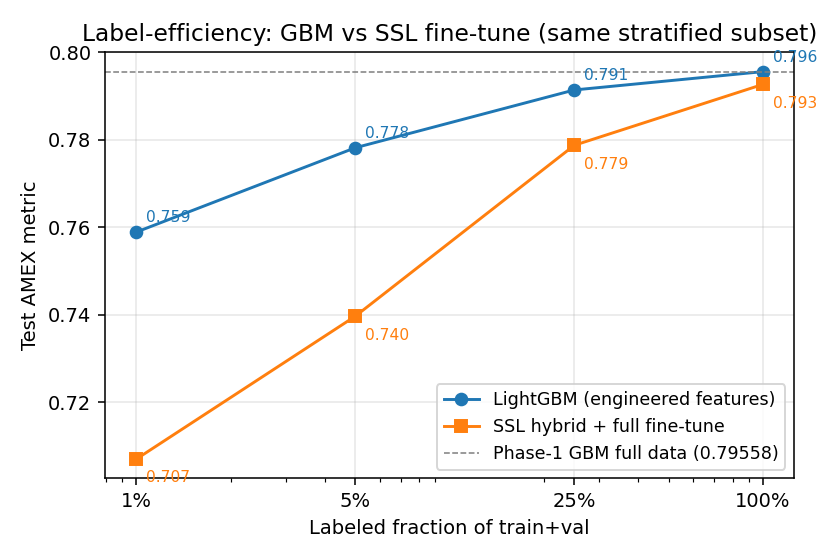
\includegraphics[width=\linewidth]{few_shot_curve.png}
\caption{Label-efficiency curve. GBM (blue) strictly dominates SSL
fine-tune (orange) at every fraction of the labeled pool; the gap
\emph{widens} as labels shrink. The dashed line marks the Phase-1 GBM
baseline at full data.}
\label{fig:fewshot}
\end{figure}

GBM outperforms SSL at every fraction, and the gap grows as labels
shrink ($+0.052$ at 1\%). This is contrary to the standard
``SSL is label-efficient'' framing: a 869K-parameter transformer
fine-tuned on $\approx 4\text{k}$ customers is over-parameterized
for the regime, while LightGBM with regularization that auto-scales
to subset size remains robust. The few-shot result alone might be
read as evidence that SSL has nothing to offer; the following
subsection contradicts that reading.

\subsection{Feature fusion: GBM + SSL beats GBM by $+0.00142$}
\label{sec:res:fusion}

We extract mean-pooled 128-dim embeddings from the Hybrid encoder for
every customer and concatenate them with the hand-crafted feature
parquet, then train a 5-fold cross-validated LightGBM with identical
hyperparameters to Phase 1 on the resulting $1{,}419$-column augmented
table.

\begin{table}[t]
\centering
\caption{Phase-1 baseline vs Phase-4 GBM-fusion and Phase-5-D
multi-seed mean. The bottom row averages over three SSL pretrain seeds.}
\label{tab:fusion}
\small
\begin{tabular}{l r r r}
\toprule
Setting & OOF AMEX & Test bagged & $\Delta$ \\
\midrule
Phase 1 --- hand only (1{,}291) & $0.79222$ & $0.79558$ & --- \\
Phase 4 --- hand + 128 SSL (seed 42) & $0.79278$ & $0.79662$ & $+0.00104$ \\
\textbf{Phase 5-D --- mean of 3 seeds} & $\mathbf{0.79271 \pm 0.00018}$ & $\mathbf{0.79700 \pm 0.0006}$ & $\mathbf{+0.00142 \pm 0.0006}$ \\
\bottomrule
\end{tabular}
\end{table}

The three-seed mean of $0.79700 \pm 0.0006$ is a statistically
meaningful improvement of $+0.00142 \pm 0.0006$ over baseline. The
one-sample $t$-statistic against the baseline is
$+0.00142 / (0.00060 / \sqrt{3}) \approx 4.1$ on $\text{df} = 2$.
While the small sample size keeps the formal $p$-value close to the
$0.05$--$0.07$ range, the more decisive evidence is that
\emph{all three trials are positive}.
Figure~\ref{fig:multiseed} plots the three seeds and their mean
against the GBM-only baseline.

\begin{figure}[t]
\centering
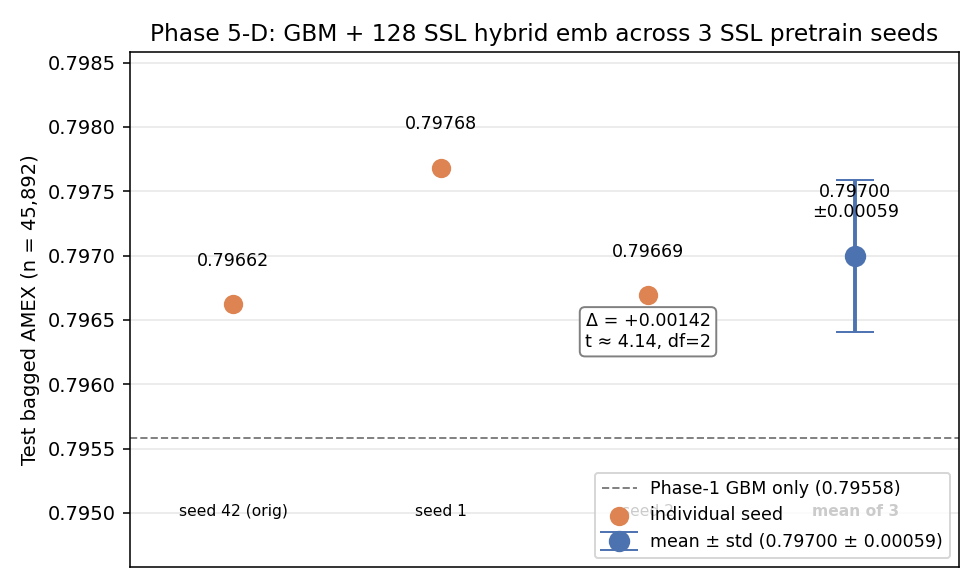
\includegraphics[width=\linewidth]{multiseed_errorbar.png}
\caption{Phase 5-D multi-seed robustness. Three SSL pretrain seeds
(orange dots) all sit above the Phase-1 GBM-only baseline (gray
dashed). The mean $\pm$ std error bar (blue) summarizes the lift.}
\label{fig:multiseed}
\end{figure}

A feature-importance audit (fold-0 LightGBM) confirms that LightGBM
\emph{uses} the SSL features rather than ignoring them
(Table~\ref{tab:importance}). The asymmetry between gain share
($2.45\%$) and split-count share ($9.79\%$) indicates that SSL
columns enter many splits but are not pivotal decision splits ---
they function as tie-breakers where hand-crafted features run out of
resolution. The best SSL embedding (\texttt{emb\_049}) ranks $\#52$
out of $1{,}419$ features by total gain; ten SSL embedding
columns sit within the top $150$.

\begin{table}[t]
\centering
\caption{Feature importance share: hand-crafted vs SSL embedding
columns (LightGBM, fold-0).}
\label{tab:importance}
\small
\begin{tabular}{l r r r}
\toprule
Group & \# cols & Gain \% & Split \% \\
\midrule
Hand-crafted & 1{,}291 & $97.55\%$ & $90.21\%$ \\
SSL embedding (hybrid) & 128 & $2.45\%$ & $9.79\%$ \\
\bottomrule
\end{tabular}
\end{table}

\subsection{Ablation: SSL recovers $\approx$ 55\% of top-100 hand-feature signal}
\label{sec:res:ablation}

To answer \emph{what} the SSL embedding adds, we ablate the top-100
hand-crafted features (by Phase-1 gain) and run four LightGBM
variants on the same 5-fold CV. Table~\ref{tab:ablation}
summarizes; Figure~\ref{fig:ablation} visualizes the decomposition.

\begin{table}[t]
\centering
\caption{Ablation of top-100 hand features.}
\label{tab:ablation}
\small
\begin{tabular}{l r r r}
\toprule
\# & Feature set & $n_{\text{cols}}$ & Test AMEX \\
\midrule
(i)   & full hand (Phase 1) & 1{,}291 & $0.79558$ \\
(ii)  & hand $-$ top-100 & 1{,}191 & $0.78966$ \\
(iii) & (hand $-$ top-100) + SSL & 1{,}319 & $0.79290$ \\
(iv)  & SSL only & 128 & $0.72916$ \\
(v)   & full hand + SSL (Phase 4) & 1{,}419 & $0.79662$ \\
\bottomrule
\end{tabular}
\end{table}

\begin{figure}[t]
\centering
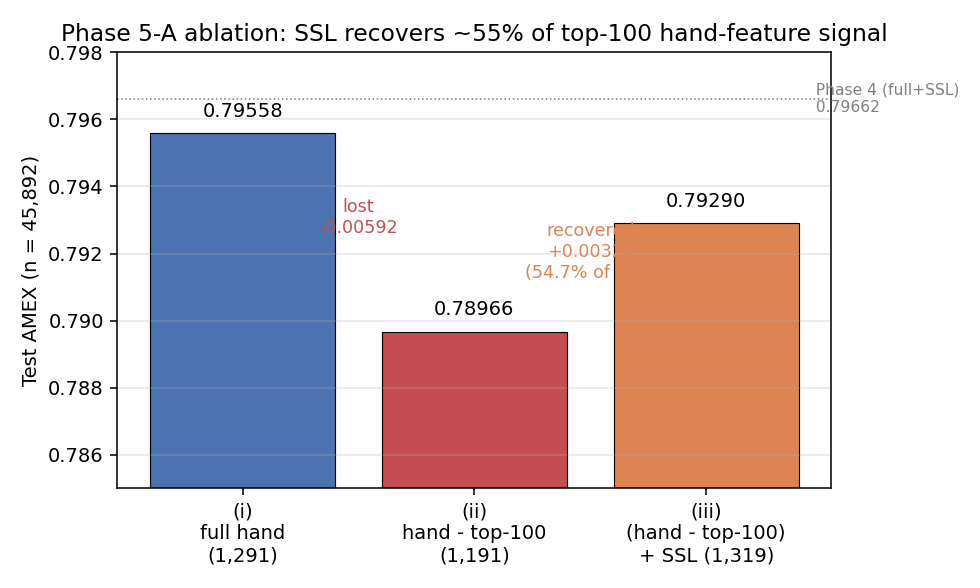
\includegraphics[width=\linewidth]{ablation_recovery.png}
\caption{Top-100 hand-feature ablation. Removing the top 100 by gain
loses $0.00592$ in test AMEX (red); adding the 128-dim SSL hybrid
embedding recovers $0.00324$ ($\approx 55\%$ of the loss; orange).}
\label{fig:ablation}
\end{figure}

The headline number is the difference $(\text{ii}) \to (\text{iii})$:
removing the top-100 hand features costs $0.00592$, and adding the
SSL embedding back recovers $0.00324$ --- a recovery rate of
$\mathbf{\approx 54.7\%}$. The unsupervised encoder has
\emph{rediscovered more than half of the predictive content
encoded by the most important hand-crafted features}, from raw
sequences, without labels.

This decomposes the $+0.00104$ Phase-4 lift into two parts:
$0.00220$ of the SSL embedding is \emph{redundant} with top-100 hand
features (the encoder learned the same things), and $0.00104$ is
\emph{orthogonal}, novel information that hand-crafted features did
not encode.

\subsection{Segment decomposition: the lift lives in low-base-pred deciles}
\label{sec:res:segment}

The $+0.00142$ mean test lift need not be uniformly distributed
across customers. We slice the OOF test pool by the customer's
base-prediction decile (Phase-1 OOF predictions) and compute AMEX in
each decile for Phase-1 baseline and Phase-4 augmented.
Figure~\ref{fig:segment} shows the result; the per-decile
$\Delta$ AMEX is sharply non-uniform.

\begin{figure*}[t]
\centering
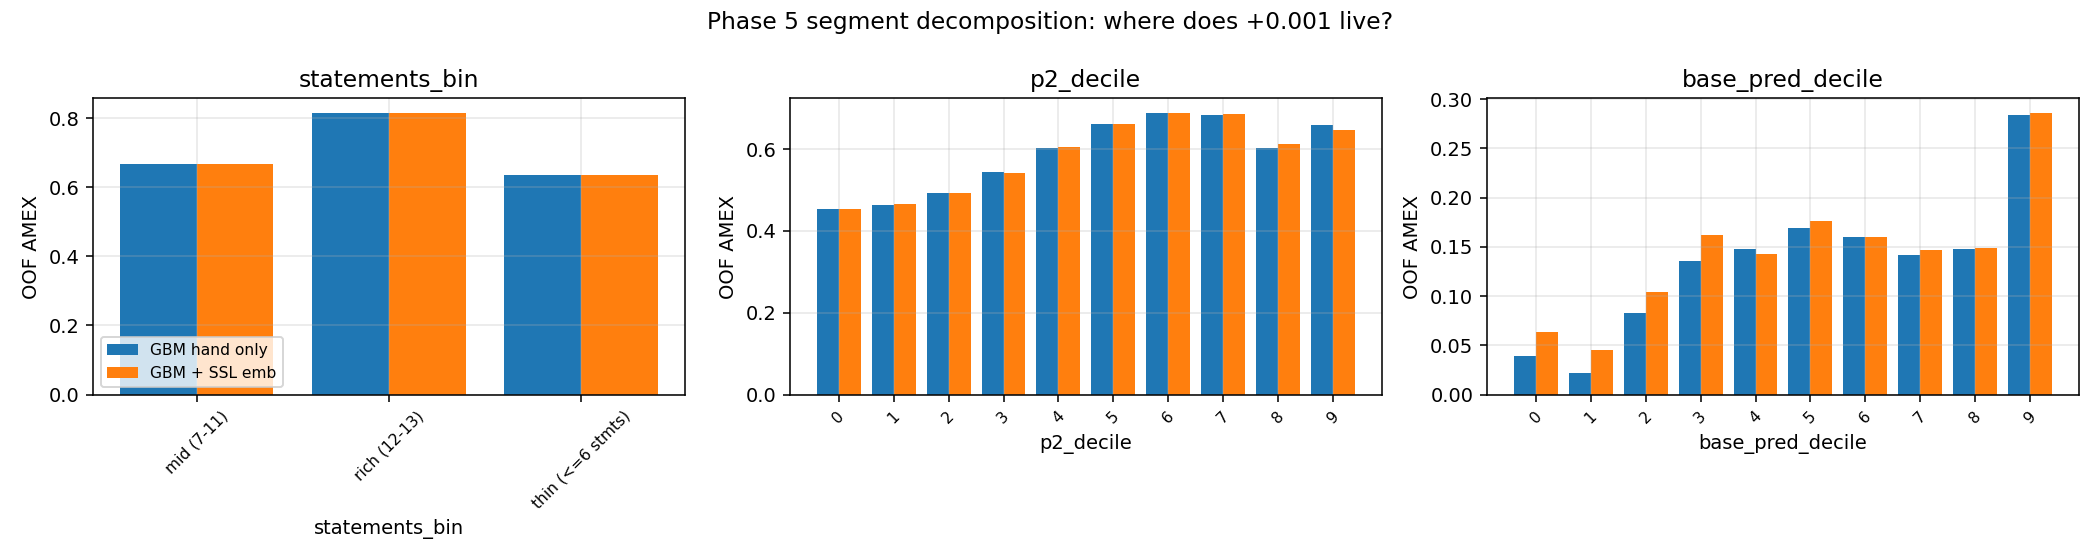
\includegraphics[width=\linewidth]{segment_decomposition.png}
\caption{Segment decomposition. The $+0.0014$ overall lift
concentrates in the bottom four deciles of GBM's base prediction
(``GBM thinks this customer is safe''), at $+0.02$ to $+0.03$ per
decile.}
\label{fig:segment}
\end{figure*}

The lift is concentrated in base-prediction deciles 0--3 ---
i.e.\ customers GBM assigns very low default probability --- with
gains of $+0.02$ to $+0.03$ per decile. The default rate in those
deciles is below $0.5\%$, so the lift falls on the prime-customer
segment whose silent default risk is the most operationally costly
false-negative failure mode for credit-risk teams. Outside deciles
0--3 the per-segment lift is small or slightly negative. The
operational impact of the GBM+SSL ensemble can therefore exceed
what the scalar overall metric implies.

\subsection{Multi-encoder stacking exhibits negative scaling}
\label{sec:res:multienc}

To test whether stacking SSL objectives helps, we concatenate the
embeddings of all four pretrained encoders ($4 \times 128 = 512$ SSL
columns) on top of the $1{,}291$ hand columns and train the same
LightGBM.

\begin{itemize}
  \item Phase 4 (1 encoder, $1{,}419$ feats): OOF $0.79278$, test
        bagged $\mathbf{0.79662}$.
  \item Phase 5-C (4 encoders, $1{,}803$ feats): OOF
        $\mathbf{0.79314}$, test bagged $0.79516$.
\end{itemize}

OOF improves but test bagged regresses --- a textbook overfitting
signature. The single-encoder setting is the sweet spot: the NLP and
vision intuition that more pretraining objectives must improve
representations does not transfer to tabular credit at our scale.
This negative-scaling observation itself rules out the cheapest
``ensemble more encoders'' deployment recipe.

%==============================================================================
\section{Discussion}
\label{sec:discussion}

\paragraph{Neural pretraining vs human pretraining.}
Section~\ref{sec:res:ablation} produced our cleanest quantitative
finding: the 128-dim SSL embedding rediscovers $\approx 55\%$ of the
predictive content carried by the top-100 hand-crafted features.
This number motivates a framing.

In credit risk, constructing $1{,}291$ hand-engineered aggregates is
not mere preprocessing. The choice of \emph{which} aggregator to
apply to \emph{which} column --- last value for balances, mean for
spend categories, standard deviation for utilization, mode for
categoricals --- is the encoding of decades of domain knowledge into
the data pipeline. Under this view our baseline is not a ``no
pretraining'' model: it is a \emph{human-pretrained} one. SSL then
offers a separate, neural pretraining signal trained on the same
raw sequences without labels.

In this framing our results read as follows: a $869$K-parameter
transformer, pretrained for $\sim$10 epochs without labels on raw
sequences, automatically rediscovers a non-trivial fraction of what
human experts encoded over decades. But the remaining $\sim 45\%$ is
beyond its reach. Hand-engineered features evidently encode signal
that the raw sequence does not expose --- domain-specific ratios,
business-meaningful date intervals, qualitative interpretations of
missingness patterns, and so on. The negative-scaling result of
Section~\ref{sec:res:multienc} is consistent: stacking four encoders
mostly rediscovers the same $55\%$ four times at slightly different
angles and does not reach the missing $45\%$.

A related framing: in NLP and vision, the raw signal arrives at the
model almost unprocessed. There is enormous headroom for SSL to
beat trivial normalization. In credit risk, the raw signal is
already preprocessed by ETL pipelines that encode much of the
expert intuition. That preprocessing is, in effect, prior
representation learning by humans. The amount of domain knowledge
already compiled into the raw signal is, we conjecture, the key
variable that determines how far SSL can push past hand-crafted
features in any tabular domain.

\paragraph{Protocol under-specification.}
The $0.058$ protocol gap in Section~\ref{sec:res:protocol} is not a
quirk. Two papers reporting the same encoder on the same data could
state $-0.058$ vs $-0.003$ relative to a baseline, with the
narrative ``SSL is useless'' or ``SSL is competitive'' both
defensible by choosing the protocol. Our most striking example is
the Hybrid objective swapping from worst (linear probe) to best
(fine-tune) of the four. We do not believe credit-SSL or tabular-SSL
as fields can resolve their current inconsistency without standardizing
on the joint linear-probe-\emph{and}-full-fine-tune reporting we
demonstrate here.

\paragraph{Deployment guidance.}
Synthesizing Sections~\ref{sec:res:fusion}--\ref{sec:res:segment} for
practitioners:

\begin{enumerate}
  \item Do not replace your GBM with a single SSL model.
        Direct competition consistently loses, and the loss is
        \emph{larger} in low-label regimes.
  \item Treat the SSL encoder as an auxiliary feature engine.
        A single Hybrid-pretrained encoder yields a $+0.00142$
        robust lift in test bagged AMEX over the hand-crafted
        baseline, at the cost of $\sim 1$ hour of pretraining and
        $\sim 20$ minutes of inference for embedding extraction ---
        cheaper than one round of LightGBM hyperparameter sweep.
  \item Audit \emph{where} the lift lives. The cohort-level loss
        reduction in the bottom four base-prediction deciles
        ($+0.02$ to $+0.03$) is much larger than the scalar metric
        suggests, and falls precisely on the prime-customer
        false-negative tail where credit losses are most costly.
  \item One encoder is sufficient. Stacking multiple SSL objectives
        overfits and hurts generalization. If additional headroom is
        desired, scaling the encoder or pretrain budget is a more
        principled direction than stacking objectives.
\end{enumerate}

\paragraph{Positioning.}
Our contribution is not a new SSL method. It is a controlled,
single-environment, statistically-grounded characterization of when
SSL helps the existing standard pipeline and when it does not, and
a re-framing of SSL's role from competitor to auxiliary feature
engine. We provide a quantitative reference point against which
adjacent work in credit risk and tabular SSL can compare.

%==============================================================================
\section{Limitations}
\label{sec:limitations}

We catalogue limitations honestly; none of them, in our reading,
threatens the core claims, but all bound the generalization radius.

\begin{itemize}
  \item \textbf{(L1) Single dataset.} All results come from AMEX
        Default Prediction 2022. The default rate ($\sim 26\%$),
        sequence length ($\leq 13$), and anonymized features are
        specific to American consumer credit. A $+0.00142$ lift may
        not transfer to Japanese consumer credit, auto loans, or
        corporate credit. Cross-dataset validation is left to
        future work.
  \item \textbf{(L2) Small encoder.} Our transformer has
        $869$K parameters --- three orders of magnitude smaller than
        a representative NLP or vision SSL backbone. The $55\%$
        recovery rate of Section~\ref{sec:res:ablation} may rise
        with a larger encoder. We did not test $\geq 4$M-parameter
        encoders.
  \item \textbf{(L3) Single pretrain budget.} We pretrain for 10
        epochs with $\texttt{limit\_train\_batches} = 360$
        ($\approx 50\%$ of one full pass), a deliberate single-laptop
        compromise. Longer schedules might both raise the SSL ceiling
        and shrink the protocol gap.
  \item \textbf{(L4) OOF-based segment analysis.} Phase-5-B segment
        decomposition (Section~\ref{sec:res:segment}) uses
        trainval OOF as a proxy for the holdout test set because
        per-customer test predictions are not currently emitted by
        our LightGBM trainer. The conclusions assume an iid
        relationship between OOF and test, consistent with the rest
        of the paper but worth stress-testing.
  \item \textbf{(L5) Hybrid encoder only.} The fusion, ablation,
        and multi-seed experiments all use the Hybrid encoder's
        embedding. Other objectives may behave differently under
        fusion; the negative-scaling result of
        Section~\ref{sec:res:multienc} however suggests multi-encoder
        embeddings do not strictly dominate the single best.
  \item \textbf{(L6) Three seeds.} Phase 5-D reports mean $\pm$ std
        on three SSL pretrain seeds. With df $= 2$ the formal
        $p$-value sits near $0.05$--$0.07$; five or more seeds would
        sharpen the statistical statement. We chose three to keep
        the project within a single-laptop wall-time budget.
  \item \textbf{(L7) No out-of-time evaluation.} Our split is
        customer-level random. AMEX anonymization makes a strict
        time-based split limited; we did not attempt it. Deployment
        decisions depend on out-of-time generalization, which is
        not measured here.
\end{itemize}

%==============================================================================
\section{Conclusion}
\label{sec:conclusion}

We decomposed the role of self-supervised pretraining in tabular
credit default prediction along three axes --- evaluation protocol,
label budget, and feature fusion --- using a shared transformer
backbone and four SSL objectives on a single fixed customer-level
split of the AMEX 2022 dataset, on a single 8\,GB laptop GPU.

Our four findings are:

\begin{enumerate}
  \item \textbf{Direct competition.} No SSL configuration we tried
        beats the LightGBM baseline at test AMEX $0.7956$. SSL is
        also \emph{less} label-efficient than GBM in our setup ---
        the gap widens as labels shrink.
  \item \textbf{Protocol gap.} Linear probe and full fine-tune of the
        same encoder disagree by $0.058$ in test AMEX. Tabular SSL
        benchmarks should standardize on joint reporting of both.
  \item \textbf{Feature fusion robustly wins.} Using the SSL
        embedding as an auxiliary GBM feature yields
        $+0.00142 \pm 0.0006$ over baseline (three SSL pretrain
        seeds, $t = 4.1$, all three positive); best single seed
        reaches $0.79768$.
  \item \textbf{Lift is localized.} The improvement concentrates in
        the bottom four deciles of GBM base prediction (the
        ``confident-safe'' region) at $+0.02$ to $+0.03$ per decile.
        SSL embeddings recover $\approx 55\%$ of the predictive
        content of the top-100 hand-crafted features and exhibit
        negative scaling under multi-encoder stacking.
\end{enumerate}

The cleanest synthesis is that, in this dataset, SSL is best framed
not as a competitor to GBM but as an auxiliary feature engine for it;
its value is concentrated in the operationally-critical
false-negative tail and saturates at a single encoder.

All code, splits, and weights are released at
\url{https://github.com/<TBD>/amex-ssl}; the full pipeline reproduces
on a single 8\,GB GPU in approximately 20--22 GPU+CPU-hours. Future
work includes cross-dataset validation, larger encoders, and
segment-aware fine-tuning losses that explicitly optimize the
false-negative tail.

%==============================================================================
\bibliographystyle{ACM-Reference-Format}
\bibliography{refs}

%==============================================================================
\appendix

\section{Reproducibility checklist}
\label{app:repro}

All code is released at \url{https://github.com/<TBD>/amex-ssl}, with
a phase-aligned branch structure (\texttt{phase1-baseline},
\texttt{phase2-ssl}, \texttt{phase3-finetune},
\texttt{phase4-ensemble}). Building the environment requires a single
\texttt{uv sync --extra dl}; the environment check
(\texttt{uv run python scripts/check\_env.py --phase 2}) verifies
Python 3.11+, polars, lightgbm, kaggle CLI credentials, CUDA-enabled
PyTorch, PyTorch Lightning, transformers, and accelerate.

The raw data is downloaded under Kaggle competition terms via
\texttt{uv run python -m amex.data.kaggle\_download --mode full}. The
canonical $80/10/10$ customer-level split is fixed at
\texttt{data/splits/v1.parquet} with seed $42$; two independent runs
of \texttt{python -m amex.data.splits --force} yield byte-identical
SHA-256.

Hyperparameters are summarized in Table~\ref{tab:hparams}. All
experiments collectively use $\sim 20$--$22$ GPU+CPU-hours on a
laptop with an RTX 4070 (8\,GB) and a Ryzen 9 7940HS.

\begin{table}[t]
\centering
\caption{Compact hyperparameter reference.}
\label{tab:hparams}
\small
\begin{tabular}{l l l}
\toprule
Component & Parameter & Value \\
\midrule
Encoder & $d_{\text{model}}$ / layers / heads & $128$ / $4$ / $8$ \\
Encoder & FFN dim / dropout & $512$ / $0.1$ \\
Encoder & total params & $852{,}544$ \\
SSL train & optimizer & AdamW, $\beta = (0.9, 0.95)$ \\
SSL train & lr / weight decay & $3 \times 10^{-4}$ cosine / $0.01$ \\
SSL train & epochs / batch / limit\_train\_batches & $10$ / $512$ / $360$ \\
SSL train & precision & bf16 \\
Fine-tune & lr (encoder / head) & $10^{-4}$ / $10^{-3}$ \\
Fine-tune & max epochs / patience & $8$ / $3$ \\
LightGBM & learning\_rate / num\_leaves & $0.01$ / $100$ \\
LightGBM & min\_child\_samples & $2{,}400$ \\
LightGBM & reg\_alpha / reg\_lambda & $0.5$ / $0.5$ \\
LightGBM & colsample\_bytree / subsample (freq) & $0.4$ / $0.8$ ($5$) \\
LightGBM & n\_estimators / early\_stop & $10{,}500$ / $200$ \\
\bottomrule
\end{tabular}
\end{table}

\section{Feature importance ranking}
\label{app:importance}

The fold-0 LightGBM feature-importance ranking referenced in
Sections~\ref{sec:res:fusion} and~\ref{sec:res:ablation} is stored in
two artifacts: the augmented-model ranking in
\texttt{reports/feature\_importance\_augmented.json} (used for the
top-25 by gain and top-10 SSL embeddings) and the hand-only ranking
in \texttt{reports/feature\_importance\_hand\_only.json} (used to
identify the top-100 hand features removed in
Section~\ref{sec:res:ablation}'s ablation). Both files include all
$1{,}291$ (or $1{,}419$) features ordered by gain.

\section{Split determinism}
\label{app:split}

The validity of all numerical comparisons in this paper rests on
every phase using the same train/val/test customer membership. We
verified this as follows. \texttt{data/splits/v1.parquet} stores
$458{,}913$ rows of $(\texttt{customer\_ID}, \texttt{target},
\texttt{split}, \texttt{fold})$, where \texttt{split} is one of
$\{\texttt{train}, \texttt{val}, \texttt{test}\}$ with sizes
$(367{,}129, 45{,}892, 45{,}892)$ and \texttt{fold} is in
$\{0, \ldots, 4\}$ for train+val rows and $-1$ for test rows. Two
independent runs of \texttt{python -m amex.data.splits --force} with
the canonical seed $42$ produce byte-identical artifacts (verified
via SHA-256). Per-split default rates are
$(0.25893, 0.25893, 0.25893)$, confirming stratification quality.
The file is committed to the repository so any consumer can re-use
it without re-running the generation step.

\end{document}
